\documentclass[12pt,margintitle,line]{res}
\usepackage[a4paper,left=1.0cm,right=4.15cm,top=1.3cm,bottom=1.5cm]{geometry}
\usepackage[utf8]{inputenc}
\usepackage[colorlinks=true,urlcolor=blue]{hyperref}
\usepackage[pdftex]{graphicx}
\usepackage{wrapfig}
\usepackage{amsmath}
\usepackage{fancyhdr}
\usepackage{amssymb}

\pagenumbering{gobble}

% specify some fonts and colors
\renewcommand{\familydefault}{\sfdefault}
\renewcommand{\sectionfont}{\scshape}
\renewcommand{\namefont}{\LARGE \bfseries}
\renewcommand{\titlefont}{\bf}
\renewcommand{\datesfont}{\bf}
\definecolor{linecolor}{RGB}{25,25,112}
\definecolor{forestgreen}{RGB}{13,55,13}
\definecolor{green}{rgb}{0.0, 0.65, 0.31}




\newcommand{\CC}{C\nolinebreak\hspace{-.05em}\raisebox{.4ex}{\scriptsize\bf +}\nolinebreak\hspace{-.10em}\raisebox{.4ex}{\scriptsize\bf +} }
\def\CC{{C\nolinebreak[4]\hspace{-.05em}\raisebox{.4ex}{\scriptsize\bf ++}}}

% override defaults
\renewcommand{\employerfont}{}

% ugly kludge: we really have to define proper subsections in the .cls file
\renewcommand{\subsection}[1]{\section{\normalfont #1}}

\setlength{\parskip}{2ex}

\hypersetup{
  pdfauthor    = {Will Wright},
  pdftitle     = {Resume: Will Wright},
  pdfsubject   = {Resume},
  pdfkeywords  = {Will Wright, Wright, Curriculum Vitae, CV, resume},
  pdfcreator   = \LaTeX{},
  pdfproducer  = \LaTeX{},
  pdfpagemode  = UseNone,% do not show thumbnails or bookmarks on opening
  pdfstartpage = 1,
}

\begin{document}

% Page number
\pagestyle{fancy}  
\fancyhf{}                  % clear default fancy headers
\renewcommand{\headrulewidth}{0.0pt}


\name{Will Wright}

\begin{resume}

% headers
\fancyhead{} % clear all header fields
\cfoot{\thepage}

% Specify the format of work entries
\begin{format}
\dates{l}\\
\title{l}\employer{r}\\
\body\\
\end{format}

%%%%%%%%%%%%%%%%%%%%%%%%%%%%%%%%%%%%%%%%%%%%%%%%%%%%%%%%%%%%%%%%%%%%%%%%%%%

% Photo

\iffalse

\begin{wrapfigure}{r}{3.24cm} 
\vspace{-3.5cm}  % Slide picture vertical up and down
\makebox[0pt][l]{
		\raisebox{-\totalheight}[0pt][0pt]{
		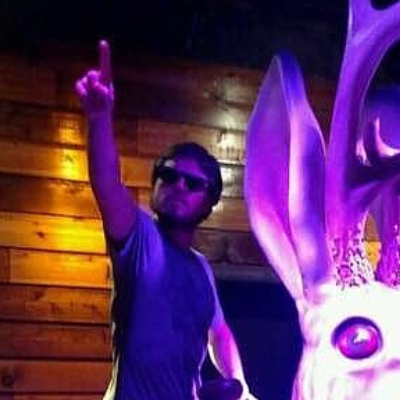
\includegraphics[width=3cm]{IMG_1443_edit.PNG}
		}
	}
\end{wrapfigure} 

\fi



%%%%%%%%%%%%%%%%%%%%%%%%%%%%%%%%%%%%%%%%%%%%%%%%%%%%%%%%%%%%%%%%%%%%%%%%%%%

\vspace{-0.2cm}

\section{Contact}
\vspace{-0.45cm}
\begin{tabbing}
Address: \= 2700 SW Hume Ct, Portland, OR 97219 \\
Mobile: \> 530-760-9363 \\
Email: \> \href{mailto:william.everett.wright@gmail.com}{\nolinkurl{william.everett.wright@gmail.com}} \\
Website: \> \url{https://will-wright.github.io} \\
GitHub: \> \url{https://github.com/will-wright} \\
\end{tabbing}

%%%%%%%%%%%%%%%%%%%%%%%%%%%%%%%%%%%%%%%%%%%%%%%%%%%%%%%%%%%%%%%%%%%%%%%%%%%


\vspace{-1.3cm}

\section{Education}

\vspace{-0.5cm}
\title{\mbox{PhD  Mathematics - University of California, Davis}}
\employer{\llap{August 2019}}
\dates{}
\begin{position}
Dissertation: 
\href{https://github.com/Will-Wright/dissertation-rapid_eigenvalue_method_for_noisy_phase_retrieval/blob/master/will_wright_dissertation.pdf} {\textsl{A Rapid Eigenvalue Method for Noisy Phase Retrieval}}
	\\
Specializations: 
	\\
$\circ$ \ Large-scale numerical methods (e.g., \href{https://github.com/Will-Wright/image-segmentation/tree/master/src}{\textsl{sparse linear algebra}})
	\\
$\circ$ \ Machine learning / deep learning applications (e.g., \href{https://github.com/Will-Wright/MNIST-CNN}{\textsl{CNNs in TensorFlow}})
	\\
$\circ$ \ Nonlinear and convex optimization
\end{position}
\\
2015-2016 - SIAM Student Chapter President


\vspace{-0.75cm}
\title{\mbox{MS  Applied Math - California State University, East Bay}}
\employer{June 2013}
\dates{}
\begin{position}
2012 - Tracewell Scholarship
	\\
2011 - Sabharwal Scholarship
\end{position}


\vspace{-0.75cm}
\title{\mbox{MA Teaching - Concordia University, Portland OR}}
\employer{June 2009}
\dates{}
\begin{position}
\end{position}


\vspace{-1.8cm}
\title{\mbox{BS  Political Science \& Philosophy - Penn State}}
\employer{Dec 2006}
\dates{}
\begin{position}
\end{position}





%%%%%%%%%%%%%%%%%%%%%%%%%%%%%%%%%%%%%%%%%%%%%%%%%%%%%%%%%%%%%%%%%%%%%%%%%%%


\vspace{-1.3cm}

\section{Internship}

\vspace{-0.5cm}
\title{Researcher \& Software Engineer - Apple}
\employer{June - Dec 2016}
\dates{}
\begin{position}
$\circ$ \ prototyped optimization methods \\
$\circ$ \ contributed performance-critical \CC \hspace{-0.02cm} code to team repository 
\end{position}



\vspace{-0.2cm}

\section{Professional Experience}

\vspace{-0.5cm}
\title{\mbox{Assistant Instructor - California State University, East Bay}}
\employer{2011 - 2013}
\dates{}
\begin{position}
\end{position}


\vspace{-1.8cm}
\title{\mbox{Middle School Teaching - Academy of Alameda, Alameda CA}}
\employer{2010 - 2011}
\dates{}
\begin{position}
\end{position}

\vspace{-1.8cm}
\title{\mbox{High School Teacher - Delta Academy, Antioch CA}}
\employer{2009 - 2010}
\dates{}
\begin{position}
\end{position}

\vspace{-1.8cm}
\title{\mbox{Underwriter - Farmers Insurance, Portland OR}}
\employer{2007 - 2008}
\dates{}
\begin{position}
\end{position}


%%%%%%%%%%%%%%%%%%%%%%%%%%%%%%%%%%%%%%%%%%%%%%%%%%%%%%%%%%%%%%%%%%%%%%%%%%%


\vspace{-1.2cm}

\section{Research Projects}

\vspace{-0.5cm}
\title{
\href{https://github.com/Will-Wright/image-segmentation} {\textsl{Image Segmentation}}
}
\employer{ 
}
\dates{}
\begin{position}

	\begin{wrapfigure}{r}{3.2cm} 
		\vspace{-0.90cm}
		\hspace{-1.95cm}
 	 	\begin{minipage}[t]{3cm}
		\makebox[0pt][l]{
			\raisebox{-\totalheight}[0pt][0pt]{
			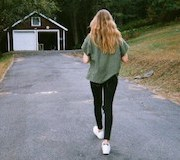
\includegraphics[width=2.2cm]{person_walking_small_edit.jpg}
			\hspace{-0.05cm}
			
\includegraphics[width=2.2cm]{person_walking_seg_edit.png}
			}
		}
  		\end{minipage} 
	\end{wrapfigure} 
	
\vspace{-1.25cm}
$\circ$ \ developed a
\href{https://github.com/Will-Wright/image-segmentation#demo-tutorial} {\textsl{faster algorithm}}
than the 
\href{http://www1.maths.lth.se/matematiklth/vision/publdb/reports/pdf/eriksson-olsson-etal-jmiv-10.pdf} {\textsl{original algorithm}}
	\\
$\circ$ \ developed a
\href{https://github.com/Will-Wright/image-segmentation/blob/master/src/GetAdjMat.py}{\textit{new sparse method}} 
for adjacency matrix,
	\\		\hspace*{0.35cm} 
requiring $\mathcal{O}(\text{pixels})$ ops vs $\mathcal{O}(\text{pixels}^2)$ in
\href{https://github.com/scikit-image/scikit-image/blob/master/skimage/future/graph/rag.py}{\textit{scikit-image}} 
\end{position}




\vspace{-0.5cm}
\title{
\href{https://github.com/Will-Wright/low-rank-opt-rapid-eig} {\mbox{\textsl{Signal/Image Processing: Phase Retrieval Denoising via Nonlinear Regression}}}
}
\employer{ 
}
\dates{}
\begin{position}
	
\vspace{-1.25cm}
$\circ$ \ developed 
\href{https://github.com/Will-Wright/low-rank-opt-rapid-eig/blob/master/adaptive_eigs_params.m}{\textit{adaptive hyperparameter selection method}}
based on 
\href{https://github.com/Will-Wright/low-rank-opt-rapid-eig#adaptive-parameter-selection-method-based-on-grid-search-results}{\textit{grid search strategy}}
	\\
$\circ$ \ \href{https://github.com/Will-Wright/low-rank-opt-rapid-eig#comparison-of-saga_sd-and-saga_sd-rapid-eig}{\textit{decreased costs and runtime}}
by 50-90\% for a recent
\href{https://arxiv.org/abs/1508.00315}{\textit{phase retrieval algorithm}}
	\\
$\circ$ \ demonstrated this algorithm is 
\href{https://github.com/Will-Wright/low-rank-opt-rapid-eig#comparison-of-saga_sd-and-wflow-for-noisy-phase-retrieval}{\textit{more accurate}}
than a highly-cited \href{https://arxiv.org/abs/1407.1065}{\textit{competitor algorithm}}
\end{position}





\vspace{-0.5cm}
\title{
\href{https://github.com/Will-Wright/lasso-quadratic-solver} {\mbox{\textsl{LASSO Regularization, Quadratic Programming}}}
}
\employer{ 
}
\dates{}
\begin{position}
	
	\begin{wrapfigure}{r}{3.2cm} 
		\vspace{-1.40cm}
		\hspace{-3.70cm}
 	 	\begin{minipage}[t]{3cm}
		\makebox[0pt][l]{
			\raisebox{-\totalheight}[0pt][0pt]{
			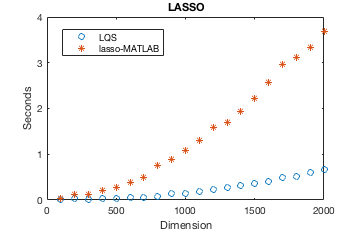
\includegraphics[width=7cm]{LQS.png}
			}
		}
  		\end{minipage} 
	\end{wrapfigure} 	
	
\vspace{-1.25cm}
$\circ$ \ 
\href{https://github.com/Will-Wright/lasso-quadratic-solver/blob/master/will_wright_qualifying_exam_proposal.pdf}{\textit{Qualifying exam proposal}} 
proved the equivalence of 
	\\ 	\hspace*{0.35cm} 
two recent methods 
(\href{https://link.springer.com/article/10.1007/s10589-017-9912-y}{\textit{smoothing}} 
and
\href{https://academic.oup.com/imajna/article/37/4/1635/3059683}{\textit{Lagrangian}})
	\\
$\circ$ \ \href{https://github.com/Will-Wright/lasso-quadratic-solver#demo-tutorial}{\textit{demonstrated}} 
this method (LQS, right) scales
	\\		\hspace*{0.35cm} 
better than built-in MATLAB software
\end{position}




%%%%%%%%%%%%%%%%%%%%%%%%%%%%%%%%%%%%%%%%%%%%%%%%%%%%%%%%%%%%%%%%%%%%%%%%%%%


\vspace{-0.2cm}

\section{Software Skills}

\title{}
\employer{}
\dates{}
\begin{position}

\vspace{-2.4cm}
\textbf{Experienced}  \ MATLAB, Python
	\\
\textbf{Intermediate} \ \CC, Git, \href{https://github.com/Will-Wright/MNIST-CNN}{\textsl{TensorFlow}}, scikit-learn, Julia
\end{position}


\section{Interests}

\vspace{-1.0cm}
\title{}
\employer{}
\dates{}
\begin{position}
Running, brewing beer, boardgames, guitar, audiobooks and podcasts (e.g., the Expanse, Stormlight Archive, Freakonomics)
\end{position}


\end{resume}
\end{document}

